%  !TeX  root  =  user_guide.tex
\chapter{Работа с данными OGC}\label{working_with_ogc}

% when the revision of a section has been finalized,
% comment out the following line:
%\updatedisclaimer

QGIS поддерживает сервисы WMS и WFS в качестве источников данных. Поддержка
WMS нативная, в то время как поддержка WFS реализовна в виде расширения.

\section{Что такое данные OGC}\index{OGC!introduction}

Open Geospatial Consortium (OGC) "--- это международная организация в состав
которой входит свыше 300 как коммерческих, так и некоммерческих,
правительственных и исследовательских организаций со всего мира. Её участники
занимаются разработкой и практической реализацией стандартов в области
геоинформационных сервисов.

Описание базовых моделей представления географических объектов и
увеличение числа спецификаций призваны удовлетворить потребности
в области сервисов, основанных на местоположении, и геопространственных
технологий, включая ГИС. Дополнительную информацию можно найти здесь
\url{http://www.opengeospatial.org/}.

Наиболее важные OGC спецификации:

\begin{itemize}[label=--]
\item \textbf{WMS} - Web Map Service
\item \textbf{WFS} - Web Feature Service
\item \textbf{WCS} - Web Coverage Service
\item \textbf{CAT} - Web Catalog Service
\item \textbf{SFS} - Simple Features for SQL
\item \textbf{GML} - Geography Markup Language
\end{itemize}

OGC-сервисы все чаще используются для обмена геопространственными
данными между различными ГИС и хранилищами данных. В настоящее время QGIS
поддерживает три из вышеперечисленных спецификации, выступая в роли SFS
(через провайдер данных PostgreSQL / PostGIS data provider, см.
Раздел~\ref{label_postgis}), WFS- и WMS-клиента.

\section{WMS
клиент}\label{sec:ogc-wms}\index{WMS!client}\index{OGC!WMS!client}\index{rasters!WMS}

\subsection{Обзор поддержки
WMS}\label{sec:ogc-wms-about}\index{WMS!client!about}

На данный момент QGIS способен выступать в роли клиента, поддерживающего WMS
серверы версий 1.1, 1.1.1 и 1.3, что было подтверждено тестами различных
публичных серверов, таких как DEMIS и JPL OnEarth.

WMS-клиент (например, QGIS) запрашивает у сервера карту заданного
охвата, содержащую определённый набор слоёв с установленной символикой и
прозрачностью. После чего WMS-сервер обращается к своему локальному хранилищу
данных, растеризует карту и отправляет её клиенту в растровом формате. В
случае QGIS таким форматом обычно является JPEG или PNG.

WMS "--- это REST (Representational State Transfer) сервис, в отличие от
полноценных Web-сервисов, что позволяет использовать URL, созданный QGIS,
во внешних приложениях, например в Web браузерах для получения таких же
изображений, что и в QGIS. Это может быть полезно при поиске неисправностей,
поскольку на рынке существуют WMS-серверы различных производителей и каждый
из них по своему интерпретирует стандарт WMS.

WMS-слои добавляются очень просто, необходимо только знать URL WMS-сервера,
иметь с ним связь и возможность использования сервером протокола HTTP в
качестве механизма передачи данных.

\subsection{Выбор WMS-серверов}\label{sec:ogc-wms-servers}\index{WMS!remote
server!selection}

При первом использовании QGIS в качетсве WMS-клиента список WMS-серверов пуст.
Нажмите кнопку \toolbtntwo{mActionAddWmsLayer}{Добавить WMS-слой} на панели
инструментов или выберите меню \mainmenuopt{Слой} \arrow \\
\dropmenuopttwo{mActionAddWmsLayer}{Добавить WMS-слой...}.

Появится окно добавления WMS-серверов \dialog{Добавить слои с сервера}.
Существует возможность автоматически добавить несколько серверов, для
этого нажмите кнопку \button{Сервера по умолчанию}. Добавится как минимум три
WMS-сервера, включая NASA (JPL). Для определения нового WMS-сервера
во вкладке \tab{Слои} выберите \button{Создать}. Затем укажите
параметры соединения с выбранным WMS-сервером как показано в таблице
\ref{tab:wms_connection_parms}:

\begin{table}[ht]\index{WMS!client!connection parameters}
\centering
 \begin{tabular}{|l|p{11cm}|}
\hline Имя & Имя соединения. Это имя будет использоваться в выпадающем
списке WMS-серверов, поэтому рекомендуется давать соединениям понятные имена. \\
\hline URL \index{WMS!URL} & URL WMS-сервера.
 Должно быть указано разрешимое имя хоста; в таком же формате, что и при
 использовании команд telnet или ping. \\
\hline Пользователь \index{WMS!authentification} & Имя пользователя для доступа к
 защищенному WMS-серверу. Этот параметр опционален. \\
\hline Пароль & Пароль для базовой аутентификации WMS-сервером. Этот параметр
опционален.\\
\hline
\end{tabular}
\caption{Параметры WMS-соединения}\label{tab:wms_connection_parms}
\end{table}

Если доступ к сервисам WMS осуществляется через прокси-сервер, необходимо
определить его параметры. Выберите меню \mainmenuopt{Установки} \arrow
\dropmenuopttwo{mActionOptions}{Параметры} и перейдите на панель \tab{Сетевые
соединения}. Задайте параметры прокси-сервера, предварительно отметив пункт \\
\checkbox{Использовать прокси-сервер для внешних соединений}.
Убедитесь в том, что в выпадающем списке \\
\dropmenuopt{Тип прокси} выбран тип, соответствующий используемому прокси-серверу.

Однажды созданное WMS соединение будет доступно и при следующем запуске
QGIS.

\begin{Tip}[ht]\caption{\textsc{URL WMS серверов}}
Убедитесь, что введен базовый URL WMS сервера. В частности он не должен
содержать таких фрагментов, как \usertext{request=GetCapabilities} или
\usertext{version=1.0.0}.\index{WMS!remote server!URL}
\end{Tip}

% in QGIS 1.1.x not needed anymore since there is a search-interface
%%% Table \ref{tab:wms_example_urls} shows some example WMS URLs to get you started.
%%% These links were last checked in April 2009, but could change at any time:
%%%
%%% %FIXME:  WMS URLs should be checked again and maybe extended in QGIS
%%% \begin{table}[ht]\index{WMS!remote server!URL!examples}
%%% \centering
%%% \caption{Example Public WMS URLs}\label{tab:wms_example_urls}\medskip
%%%  \begin{tabular}{|l|l|}
%%% \hline \textbf{Name}        & \textbf{URL} \\
%%% \hline Atlas of Canada      & http://atlas.gc.ca/cgi-bin/atlaswms\_en? \\
%%% \hline DEMIS                & http://www2.demis.nl/wms/wms.asp?wms=WorldMap\& \\
%%% \hline Geoscience Australia & http://www.ga.gov.au/wms/getmap?dataset=national\& \\
%%% \hline NASA JPL OnEarth     & http://wms.jpl.nasa.gov/wms.cgi? \\
%%% % \hline QGIS Users           & http://qgis.org/cgi-bin/mapserv?map=/var/www/maps/main.map\& \\
%%% \hline QGIS Users           & http://linfiniti.com:8080/geoserver/wms? \\
%%% \hline
%%% \end{tabular}
%%% \end{table}
%%%
%%% An exhaustive list of WMS servers can be found at \url{http://wms-sites.com}.

\subsection{Загрузка WMS-слоев}\label{sec:ogc-wms-layers}\index{WMS!client!layers}

Как только были заданы параметры WMS-соединения, можно нажать кнопку
\button{Подключиться} для получения доступа к содержимому выбранного
сервера, которое включает формат изображения, слои, стили слоев и
информацию о проекциях. Поскольку это сетевая операция, то скорость ее
исполнения зависит от качества связи с WMS-сервером. Процесс загрузки
данных визуализируется в левом нижнем углу окна добавления WMS-слоя.

Содержимое экрана должно напоминать Рисунок~\ref{fig:connection_wms}, на
котором представлены данные, доступные на WMS срвере NASA JPL OnEarth.

\begin{figure}[ht]
  \centering
  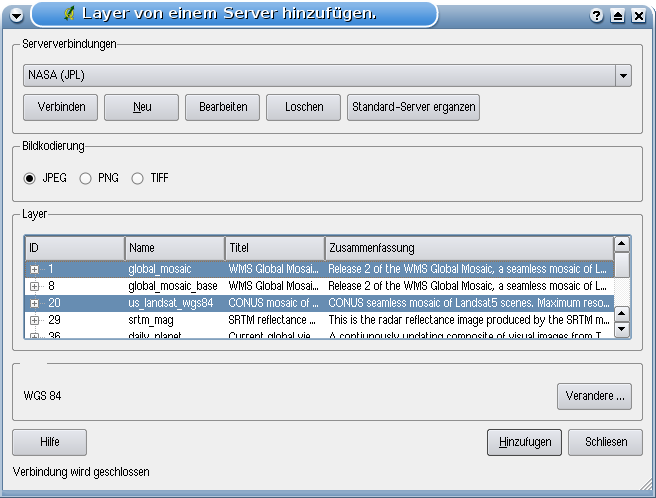
\includegraphics[clip=true,width=0.6\textwidth]{connection_wms}
  \caption{Диалоговое окно добавления WMS-сервера, представлены доступные слои
  \nixcaption}\label{fig:connection_wms}
\end{figure}

\minisec{Формат изображений}

Панель \tab{Формат изображения} содержит список форматов,
поддерживающихся одновременно как сервером, так и клиентом.
Выберите формат, удовлетворяющий требованиям к точности изображния.

\begin{Tip}[ht]\caption{\textsc{Формат изображения}}
Обычно WMS-серверы предлагают на выбор один из двух форматов "--- JPEG или PNG.
JPEG "--- это формат, использующий алгоритм сжатия с потерями, в то время
как PNG "--- без потерь.

Используйте JPEG, если предполагается, что данные полученные по WMS
будут представлять собой фотографии природы и/или вам не принципиально
небольшое снижение качества изображений. Использование JPEG позволяет
приблизительно в 5 раз снизить объём передаваемой информации по сравнению
с PNG.

Используйте PNG, если хотите получить точное воспроизведение оригинальных
данных и вас не беспокоит объём передаваемой информации. \index{WMS!image encoding}
\end{Tip}

\minisec{Параметры}

Панель\tab{Параметры} содержит текстовое поле, где можно указать имя
WMS-слоя. Это имя будет отображено в списке слоев по завершении загрузки.

Если URL OnlineRessource в ответе GetCapabilities отличается от заданного в
параметрах соединения URL, QGIS спросит о том, какой URL использовать.
В зависимости от вашего выбора QGIS отметит один из переключателей. Также это
можно сделать в любой момент самостоятельно с помощью переключателей
\checkbox{Игнорировать GetMap URL} и \checkbox{Игнорировать GetFeatureInfo URL}.

\minisec{Слои} \label{ogc-wms-layers}

Вкладка \tab{Слои} содержит список доступных слоев на выбранном WMS-сервере.
Можно заметить, что некоторые слои представляют собой раскрывающийся список,
это свидетельствует о том, что данные слои можно отобразить с использованием
различных стилей.

Можно выбрать несколько слоёв за раз, но при этом каждый из них с
использованием только одного стиля. Если выбрано несколько слоёв, то
они будут объединены на WMS-сервере и сразу переданы QGIS.

\begin{Tip}[ht]\caption{\textsc{Порядок WMS-слоёв}}
В данной версии QGIS WMS-слои отрисовываются сервером путём наложения
друг на друга в порядке, представлнном во вкладке \tab{Слои}, начиная с конца
списка. Если нужно поменять порядок отрисовки слоёв, воспользуйтесь вкладкой
\tab{Порядок слоёв}.
\index{WMS!remote server!layer ordering}
\end{Tip}

\minisec{Прозрачность}\label{ogc-wms-transparency}

Прозрачность слоёв жестко прописана в коде и всегда включена для тех
слоёв, которые её поддерживают.

\begin{Tip}[ht]\caption{\textsc{Прозрачность WMS-слоёв}}
Доступность прозрачности WMS-слоёв зависит от используемого формата изображения:
так PNG и GIF поддерживают прозрачность, в то время как JPEG "--- нет.
\index{WMS!layer transparency}
\end{Tip}

\minisec{Система координат}
\index{WMS!CRS}
\index{WMS!coordinate reference system}
\index{OGC!CRS}
\index{OGC!coordinate reference system}
\index{Projections!WMS}
\index{Projections!CRS}
\index{Projections!coordinate reference system}
\index{CRS}
\index{coordinate reference system}
\index{SRS}
\index{Projections!SRS}

Система координат (CRS, Coordinate Reference System) "--- проекция в
терминологии OGC.

В зависимости от настроек WMS-сервера, каждый слой может быть доступен в
нескольких проекциях. Можно заметить, что величина \textsl{x}
на панели \textsl{Система координат (доступно x)}
изменяется при выборе слоёв из списка вкладки \tab{Слои}.

Для выбора системы координат нажмите кнопку \button{Изменить...}, появится
окно, подобное тому, что представлено на Рисунке~\ref{fig:projections} в
Разделе~\ref{label_projstart}. Основное отличие WMS версии данного окна
состоит в том, что оно содержит только те системы координат, которые
поддерживаются WMS-сервером.

\begin{Tip}[ht]\caption{\textsc{Системы координат WMS}}
Рекомендуется всегда добавлять WMS-слой первым в проект. Это позволит в
дальнейшем использовать его проекцию при добавлении в проект других слоёв.
Приведение слоёв к проекции проекта достигается путём использования
преобразования координат <<на лету>> (см. Раздел~\ref{sec:projection-specifying}).
В текущей версии QGIS в случае добавления в проект WMS-слоя не первым и
установки ему проекции, отличной от проекции проекта, возможны
непредсказуемые последствия.
\end{Tip}

%
% server-search tab.
%
\subsection{Поиск серверов}
\label{sec:serversearch}
\index{WMS!serversearch}
\index{WMS!search}
\index{OGC!search}

QGIS позволяет осуществлять поиск WMS-серверов. На Рисунке~\ref{fig:searchtab}
показана вкладка \tab{Поиск серверов} диалогового окна
\dialog{Добавить слои с сервера}.

\begin{figure}[ht]
  \centering
  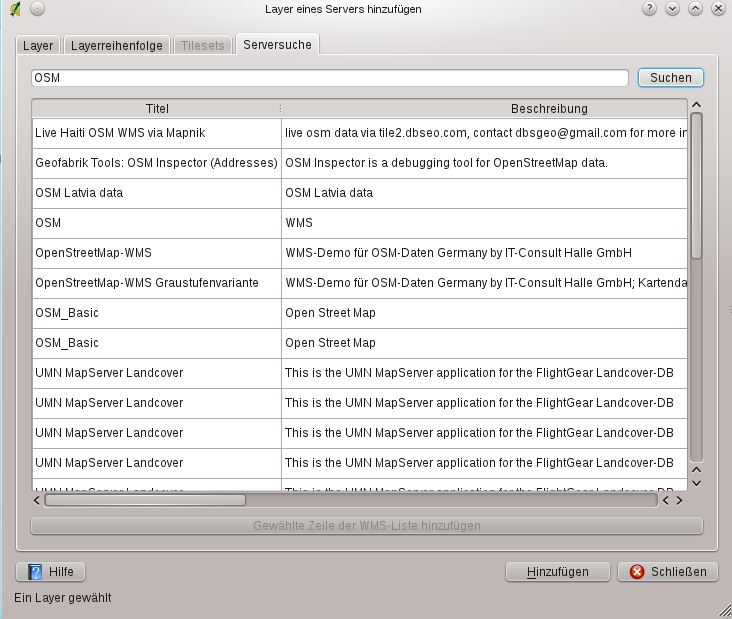
\includegraphics[clip=true,width=0.6\textwidth]{wms_server-search}
  	\caption{Вкладка поиска WMS-серверов по ключевым словам
  	\nixcaption}\label{fig:searchtab}
\end{figure}

Для начала процедуры поиска необходимо указать в текстовом поле ключевые
слова и нажать кнопку \button{Поиск}.

После завершения поиска результаты будут отображены в виде списка,
расположенного под текстовым полем.

Просмотрите получившийся список и выберите нужную строку. Для визуализации
слоёв с выбранного сервера нажмите кнопку \button{Добавить выбранный сервер в
список} и вернитесь обратно во вкладку \tab{Поиск серверов}.

QGIS автоматически обновляет список серверов, добавляя в него выбранный
WMS-сервер и делая его активным.

Пользователю остаётся только получить список слоёв с сервера, нажав кнопку
\button{Подключиться}.

Эта возможность очень удобна в случае необходимости поиска карт по
ключвым словам.

Фактически это фронт-энд к API \url{http://geopole.org}.

%
% Tilesets
%
\subsection{Мозаики}\label{sec:tilesets}
\index{WMS!tileset}
\index{WMS!WMS-C}

% Указанный URL недоступен
При использовании WMS-C (Cached WMS) сервисов, подобных
\url{http://labs.metacarta.com/wms-c/Basic.py}, становится активной вкладка
\tab{Мозаики}, в которой представлена такая информация, как размер
тайлов, поддерживаемые форматы и проекции.

В сочетании с этой возможностью удобно использовать переключатель масштаба
\mainmenuopt{Вид} \arrow \\
\dropmenuopt{Уровень детализации}, отражающий доступные масштабы
тайл-сервера и обладающий удобным механизмом их смены.
%
% Identify
%
\subsection{Использование инструмента определения
объектов}\label{sec:ogc-wms-identify}
\index{WMS!identify}
\index{identify!WMS}
\index{WMS!GetFeatureInfo}

Если слой, предоставляемый WMS-сервером, даёт возможность осуществления
запросов, то появляется возможность использовать инструмент
\toolbtntwo{mActionIdentify}{Определить объекты} для получения информации о
пикселях карты. При каждой попытке получения такой информации происходит
обращение к WMS-серверу.

Результат запроса представялется в виде простого текста,
а его форматирование определяется настройками того или иного WMS-сервера.

\subsubsection{Просмотр
свойств}\label{sec:ogc-wms-properties}\index{WMS!properties}
\index{rasters!properties}

Для просмотра свойств WMS-сервера добавьте в проект слой с этого сервера, в
списке слоёв щелкните на нём правой кнопкой мыши и выберите \button{Свойства}.

\minisec{Метаданны}\label{sec:ogc-wms-properties-metadata}
\index{rasters!metadata}
\index{WMS!metadata}
\index{WMS!capabilites}

Вкладка \tab{Метаданные} содержит богатую информацию о
WMS-сервере, полученную из ответа Capabilities.

Определения большинства параметров можно найти в описании стандарта WMS
\cite{OGCWMS010101web}, \cite{OGCWMS010300web}, представим некоторые из них:

\begin{itemize}[label=--]
\item \textbf{Свойства сервера}

\begin{itemize}[label=--]
\item \textbf{Версия WMS}          "--- Версия WMS, поддерживаемая сервером.

\item \textbf{Форматы изображения} "--- Список MIME-типов, поддерживаемых
                                       сервером. QGIS доступны любые форматы, с
                                       поддержкой которых была собрана
                                       библиотека Qt, обычно это
                                       \texttt{image/png} и \texttt{image/jpeg}.

\item \textbf{Форматы запроса}     "--- Список MIME-типов, в которых сервер может
                                       отдавать ответы на запросы к слою. В
                                       настоящее время QGIS поддерживает только
                                       \texttt{text-plain}.

\end{itemize}

\item \textbf{Свойства слоя}

\begin{itemize}[label=--]
\item \textbf{Выбранные слои}        "--- Показывает был или не был выбран слой
                                         при добавлении сервера в проект.

\item \textbf{Видимость}             "--- Определяет включена или отключена
                                         видимость слоя в списке слоёв. (Не
                                         используется в текущей версии QGIS.)

\item \textbf{Можно определять}      "--- Возможно или нет осуществлять
                                         запросы к слою с помощью инструмента
                                         идентификации.

\item \textbf{Может быть прозрачным} "--- Показывает доступна или нет
                                         возможность рендеринга слоя с
                                         поддержкой прозрачности. Текущая версия
                                         QGIS всегда использует прозрачность,
                                         если это значение равно \textsl{Да} и
                                         формат изображения поддерживает
                                         прозрачность.
% BM: doesn't seem to work?
%                                    (see Section
%                                    \ref{ogc-wms-transparency}
%                                    ).
                                    .

\item \textbf{Можно увеличивать}    "--- Доступна или нет возможность
                                        увеличения слоя на стороне сервера.
                                        Текущая версия QGIS подразумевает, что
                                        этот параметр для любого слоя установлен
                                        в значение \textsl{Да}. Не отвечающие
                                        данному требованию слои могут быть
                                        отрисованы некорректно.

\item \textbf{Количество каскадов}  "--- Одни WMS-серверы могут работать как
                                        прокси-серверы для других. Эта запись
                                        показывает сколько раз запрос к данному
                                        серверу был проброшен на другие WMS
                                        серверы до моментв получения результата.

\item \textbf{Фикс. ширина, Фикс. высота}
                                   "--- Установлен или нет фиксированный
                                       размер слоя в пикселях. Текущая версия
                                       QGIS подразумевает, что этот параметр для
                                       любого слоя не установлен. Не отвечающие
                                       данному требованию слои могут быть
                                       отрисованы некорректно.

\item \textbf{Рамка WGS 84}        "--- Ограничивающий прямоугольник
                                       слоя в координатах WGS 84. Некоторые
                                       WMS-серверы некорректно устанавливают значение данного параметра
                                       (например, используются координаты UTM).
                                       В таком случае слой может быть отрисован
                                       на очень высоком зуме. О таких ошибках
                                       следует сообщать администратору WMS-сервера,
                                       который сможет устранить их
                                       путём редактирования элементов WMS XML
                                       \texttt{LatLonBoundingBox},
                                       \texttt{EX\_GeographicBoundingBox} или
                                       CRS:84 \texttt{BoundingBox}.

\item \textbf{Доступен в CRS}      "--- Проекции, в которых может быть отрисован
                                       слой WMS-сервером. Перечислены в нативном
                                       для WMS формате.

\item \textbf{Доступен в стилях}   "--- Стили в которых может быть отрисован слой
                                       WMS-сервером.

\end{itemize}

\end{itemize}


\subsection{Ограничения WMS-клиента}\label{sec:ogc-wms-limits}\index{WMS!client!limits}

Не все возможности WMS-клиента были включены в текущую версию
QGIS. Рассмотрим наиболее значимые:

\minisec{Редактирование свойств WMS-слоя}
\index{WMS!layer settings!editing}

После завершения процедуры \toolbtntwo{mActionAddWmsLayer}{Добавить WMS-слой},
изменить настройки слоя невозможно.

Данное ограничение обходится путём полного удаления слоя и повторного
его добавления с новыми настройками.

\minisec{Защищённые WMS-серверы}
\index{WMS!remote server!authentication}
\index{WMS!remote server!basic authentification}

В настоящее время поддерживается работа как с публичными, так и с защищёнными
WMS-серверами. Доступ к защищённым WMS-серверам можно получить посредством
прохождения публичной аутентификации.
Имя пользователя и пароль (опционально) задаются при добавлении WMS-сервера.
За подробностями обратитесь к Разделу~\ref{sec:ogc-wms-servers}.

\begin{Tip}[ht]\caption{\textsc{Доступ к защищённым слоям OGC}}
Если необходимо получить доступ к защищённым слоям, требующим прохождения
аутентификации отличной от базовой, то следует воспользоваться прозрачным
прокси-сервером InteProxy, поддерживающим различные методы
аутентификации. Дополнетельную информацию можно найти в руководстве
InteProxy, расположенном по адресу
\url{http://inteproxy.wald.intevation.org}.
\index{WMS!secured layers!}\index{OGC!Authentication}
\end{Tip}

%
% WFS-client
%
\section{Клиент WFS}\label{sec:ogc-wfs}

В QGIS работа с WFS и обычными векторными слоями практически неотличима.
Можно выделять и получать информацию об объектах, просматривать таблицу
атрибутов. Единственное отличие заключается в том, что отсутствует возможность
редактирования (данная возможность обеспечивается протоколом WFS-T и ожидается
в QGIS в ближайшее время). Чтобы включить расширение для работы с WFS, откройте
\mainmenuopt{Модули} \arrow \dropmenuopttwo{mActionShowPluginManager}{Управление
модулями...}, отметьте пункт \checkbox{Модуль WFS} и нажмите
\button{OK}.

Новая кнопка \toolbtntwo{mIconAddWfsLayer}{Добавить слой WFS} появится на той
же панели инструментов, что и кнопка добавления WMS-слоя. Нажмите на неё,
откроется диалоговое окно. Добавление слоя WFS очень похоже на добавление слоя
WMS. Отличие только в том, что отсутствуют предопределенные WFS-серверы.

\subsubsection{Добавление слоя WFS}

В качестве примера будем использовать WFS сервер DM Solutions:
\begin{verbatim}
http://www2.dmsolutions.ca/cgi-bin/mswfs_gmap?VERSION=1.0.0&SERVICE=
wfs&REQUEST=GetCapabilities
\end{verbatim}

\begin{enumerate}
  \item Убедитесь, что расширение для работы с WFS включено; если нет, то
  откройте менеджер модулей QGIS и включите его
  \item Нажмите кнопку
  \toolbtntwo{mIconAddWfsLayer}{Добавить слой WFS}
  на панели инструментов
  \item Нажмите \button{Создать}
  \item Укажите \inputtext{{}Имя}{DM Solutions} в качестве имени
  \item Введите URL (см. предыдущую страницу)
  \item Нажмите \button{OK}
  \item В выпадающем списке выберите \selectstring{{}Соединения с серверами}{DM
  Solutions}
  \item Нажмите \button{Подключиться}
  \item Дождитесь заполнения списка доступных слоев
  \item Выберите слой \clicklistitem{park}
  \item Чтобы добавить слой на карту, нажмите \button{OK}
  \item Дождитесь загрузки объектов
\end{enumerate}

Отметим, что расширение для работы с WFS использует настройки
прокси-сервера, если таковые были заданы.

\begin{figure}[ht]
  \centering
  	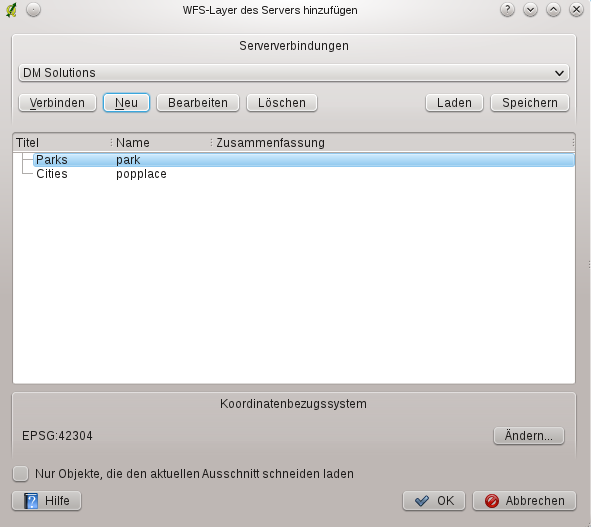
\includegraphics[clip=true,width=0.45\textwidth]{connection_wfs}
  	\caption{Добавление слоя WFS \nixcaption}\label{fig:wfs_dmsolutions}
\end{figure}

Если пункт \checkbox{Ограничить запрос объектов текущим охватом}
не отмечен, то QGIS получает все объекты с WFS-сервера. Если необходимо
загрузить только те объекты, которые попадают в интересующий охват,
то нужно изменить масштаб до необходимого фрагмента и запросить WFS-слой, при
этом убедившись в том, что отмечен вышеозначенный пункт. В результате
чего в строку запроса будет добавлен параметр BBOX, значение которого будет
соответствовать текущему охвату. Эта возможность очень полезна в тех случаях,
когда нужно получить всего \textbf{несколько} объектов из большого набора
данных.

Процесс загрузки слоя визуализируется в левом нижнем углу главного окна
QGIS. По окончании загрузки можно выделять и получать информацию об
интересующих объектах, просматривать таблицу атрибутов.

Помните, что расширение WFS наиболее корректно работает с WFS-серверами,
созданными на базе MapServer. При работе с серверами, построенными на базе
другого ПО, возможно непредсказуемое поведение. Улучшение модуля WFS
ожидается в будущих версиях.

Другими словами, на настоящий момент поддерживается только WFS версии 1.0.0.
Тестирование расширения на WFS-серверах, использующих другие версии
протокола, не проводилось. При возникновении проблем в таких ситуациях
не стесняйтесь и задавайте вопросы разработчикам расширения.
Пожалуйста, обратитесь к Разделу~\ref{label_helpsupport} для получения
дополнительной информации о листах рассылки.

\begin{Tip}[htb]\caption{\textsc{Поиск WFS серверов}}
Дополнительные WFS-серверы можно найти, используя Google
или любую другую поисковую систему. Существует множество списков, содержащих
URL WFS-серверов, некоторые из которых поддерживаются, а некоторые уже нет.
\index{WFS!remote server!}
\end{Tip}

\begin{Tip}[htb]\caption{\textsc{Доступ к защищенным WFS серверам}}
В диалоговом окне \dialog{Создание нового WFS-соединения} поддержка
аутентификации WFS-соединения не реализована. Тем не менее для доступа к
WFS-ресурсам, требующим прохождения аутентификацию, можно воспользоваться
сервисом (\url{http://inteproxy.wald.intevation.org}).
\index{WFS!authenticate remote server!}
\index{WFS!secured WFS server!}
\end{Tip}

\FloatBarrier
